\chapter{PROJETO E IMPLEMENTAÇÃO DA APLICAÇÃO PROPOSTA}

A aplicação Desconecta foi projetada adotando o paradigma de \emph{\textit{Backend-as-a-Service}} (\textit{BaaS}), com o objetivo de simplificar a arquitetura e reduzir a complexidade de infraestrutura. Nesse modelo, eliminou-se a necessidade de um servidor intermediário dedicado, transferindo a responsabilidade de \textit{backend} para serviços gerenciados em nuvem.

A arquitetura foi definida com base em dois componentes principais. O primeiro consiste em um aplicativo para dispositivos móveis, responsável pela interface gráfica, pelo fluxo de navegação e por parte da lógica de negócio executada no cliente. O segundo componente é o ecossistema \textit{Firebase}, mantido pelo \textit{Google}, que provê os serviços de \textit{backend} necessários para o funcionamento do sistema.

O aplicativo \textit{mobile} foi implementado como ponto central de interação do usuário com as funcionalidades propostas, incluindo monitoramento de tempo de tela, métricas de uso e recursos sociais baseados em gamificação. Diferentemente de arquiteturas tradicionais baseadas em \textit{APIs REST}, optou-se por realizar a integração direta com os serviços do \textit{Firebase} por meio de \textit{SDKs} oficiais. Essa decisão arquitetural reduziu a necessidade de implementação de \textit{endpoints} próprios e simplificou o fluxo de comunicação entre cliente e \textit{backend}.

No contexto da infraestrutura, o \textit{Firebase} foi configurado como núcleo de gerenciamento da aplicação. A persistência de dados foi implementada por meio do \textit{Cloud Firestore}, que permite armazenamento estruturado em documentos e coleções. O processo de autenticação foi realizado utilizando o módulo de autenticação do próprio \textit{Firebase}, garantindo controle de acesso seguro e gerenciamento de sessões. 

Para armazenamento de mídias, foi utilizado o serviço de \textit{Cloud Storage}. O disparo de notificações \emph{push} foi configurado com suporte a eventos e regras definidas no \textit{backend} gerenciado.

Essa abordagem arquitetural garantiu alta disponibilidade, escalabilidade automática e o mais importante para o \textit{MVP}, agilidade no desenvolvimento. Com isso, o esforço pôde ser direcionado prioritariamente à experiência do usuário, ao refinamento do fluxo de uso e à implementação de funcionalidades relacionadas à redução do tempo de tela no ambiente móvel.


\section{Arquitetura Lógica}
A arquitetura do sistema possuí dois elementos principais. O primeiro é a interface gráfica, o aplicativo móvel, nele que o usuário irá interagir para ter acessos às funcionalidades e também será responsável pelo processamento. O segundo é o banco de dados remoto, ele ficará responsável por guardar todas as informações dos usuários. O diagrama pode ser observado na Figura 11. Na seção 4.5 detalharemos mais a arquitetura, explicando minuciosamente os componentes.
\begin{figure}[H]
    \centering
    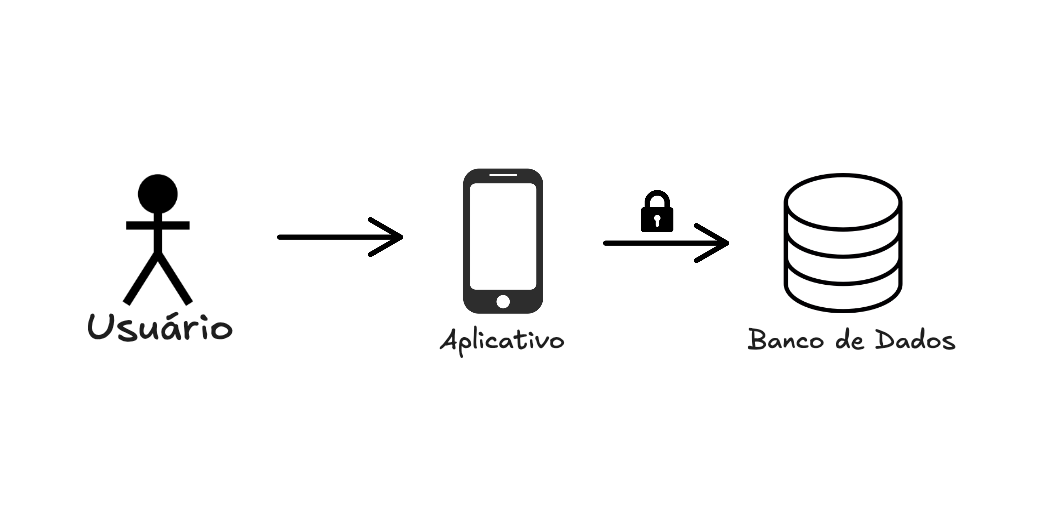
\includegraphics[width=0.8\textwidth]{figuras/arquitetura-logica.png}
    \caption{Arquitetura Lógica}
    \label{fig:Arquitetura}
\end{figure}


\section{Funcionalidades do aplicativo e tecnologias de implementação}
As funcionalidades do aplicativo foram agrupadas em quatro categorias: (i) Monitoramento de Uso de Tela; (ii) Alertas com Notificação e Metas Pessoais; (iii) Perfil e Personalização; (iv) Interação Social e Gamificação.

(i) \textbf{Perfil e Personalização}: cada usuário terá um perfil público, em que poderá cadastrar informações como nome, foto e uma breve descrição. Esses dados ficam armazenados de forma segura no \textit{Firebase}\footnote{Firebase. Disponível em: \url{https://firebase.google.com/}. Acesso em: 18 fev. 2026.} e as imagens no \textit{Firebase Storage}\footnote{Firebase Storage. Disponível em: \url{https://firebase.google.com/products/storage}. Acesso em: 18 fev. 2026.}. A escolha desse ecossistema se justifica por integrar autenticação, banco de dados e armazenamento de arquivos em um único serviço gerenciado, com escalabilidade automática e plano gratuito suficiente para o escopo deste \textit{MVP}.

(ii) \textbf{Monitoramento de Uso de Tela}: abrange a coleta de dados referente ao uso do dispositivo e aplicativos de terceiros. Inclui a contagem de desbloqueios de tela e o registro manual de informações quando a automação não for possível por restrições do sistema operacional.

(iii) \textbf{Alertas com Notificação e Metas Pessoais}: categoria responsável pelo gerenciamento de metas de tempo de tela (individuais ou de grupo). A entrega das notificações é realizada através do \textit{Firebase Cloud Messaging} (\textit{FCM}), permitindo alertas em tempo real.

(iv) \textbf{Interação Social e Gamificação}: funcionalidade central do aplicativo, englobando grupos de tempo de tela e \textit{rankings}. Utiliza a capacidade de sincronização em tempo real do \textit{Firebase} para atualizar \textit{rankings} e desafios estaduais ou regionais para todos os membros.

\subsection{ Telas do Aplicativo}
A estrutura de telas do aplicativo Desconecta foi planejada para refletir um fluxo lógico que se inicia no \textit{onboarding} e na configuração de primeiro acesso. As interfaces foram hierarquizadas em cinco eixos principais de funcionalidade, representados visualmente como as colunas do mapa de navegação: Grupos de Amigos, Desafios Públicos, Home Dinâmica, Estatísticas Pessoais e Configurações. Essa organização serviu de guia para a programação das rotas e para a definição das áreas clicáveis, permitindo que o usuário transite entre a visualização de dados de uso, como o tempo por categoria de \textit{app}, e as interações sociais de forma intuitiva. A listagem completa de telas, detalhando as funções de bloqueio por horário e gamificação, está disponível no Apêndice D.

\begin{figure}[htbp]
    \centering
    \caption{Fluxo de Telas}
    \label{fig:fluxo-telas}
    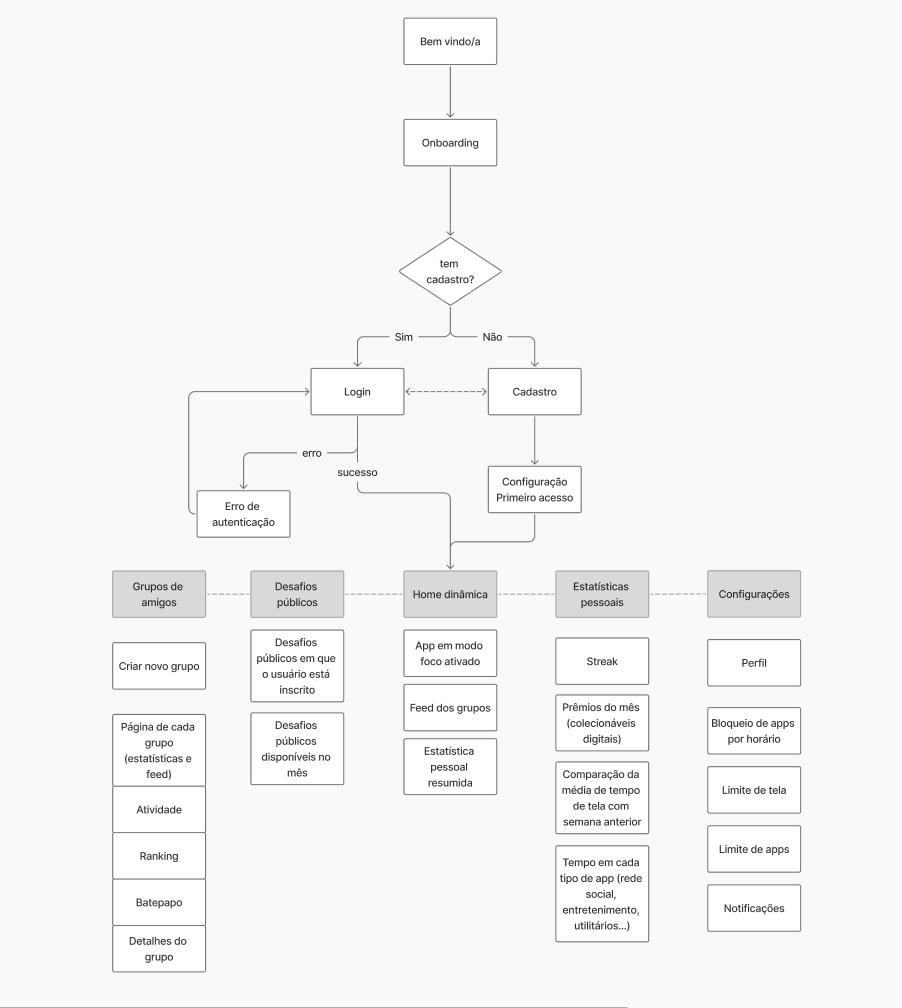
\includegraphics[width=1\textwidth]{figuras/telas.jpeg}
\end{figure}

\subsection{ Requisitos Funcionais}
Esta subseção descreve as funcionalidades implementadas no protótipo, associando-as aos requisitos funcionais definidos no Capítulo 3.
\begin{table}[H]
\centering
\caption{Quadro 1 - Requisitos Funcionais de (i) Perfil
e Personalização}
\begin{tabularx}{\textwidth}{|c|l|X|}
\hline
\rowcolor{verdeclaro}
\textbf{RF} & \textbf{REQUISITO} & \textbf{DESCRIÇÃO} \\ \hline

1 & Criar Conta &
Deve ser possível criar uma conta de usuário do aplicativo utilizando o \textit{Firebase Authentication}. \\ \hline

2 & Editar Dados Pessoais &
Deve ser possível editar dados pessoais em sua conta de usuário, como nome e descrição, mas não o email. \\ \hline

3 & Enviar Foto de Perfil &
Deve ser possível enviar uma foto de perfil nova, caso haja uma cadastrada, substituir a anterior. \\ \hline

4 & Autenticação &
Deve ser possível se autenticar no aplicativo por meio de uma conta Google, provedor de autenticação atualmente implementado. \\ \hline

5 & Fazer Logout &
Deve ser possível fazer \textit{logout} do aplicativo, voltando para tela de \textit{login}. \\ \hline

\end{tabularx}
\end{table}


\begin{table}[H]
\centering
\caption{Quadro 1 - Requisitos Funcionais de (ii) Monitoramento de Uso de Tela}
\begin{tabularx}{\textwidth}{|c|l|X|}
\hline
\rowcolor{verdeclaro}
\textbf{RF} & \textbf{REQUISITO} & \textbf{DESCRIÇÃO} \\ \hline

1 & Monitoramento de Uso de Tela &
Deve ser possível monitorar o tempo de tela e dos aplicativos do usuário. \\ \hline

2 & Cadastro de Monitoramento de Uso de Tela &
Deve ser possível cadastrar uma imagem do monitoramento de uso de tela. \\ \hline

\end{tabularx}
\end{table}


\begin{table}[H]
\centering
\caption{Quadro 1 - Requisitos Funcionais de (iii) alertas com Notificação e Metas Pessoais}
\begin{tabularx}{\textwidth}{|c|l|X|}
\hline
\rowcolor{verdeclaro}
\textbf{RF} & \textbf{REQUISITO} & \textbf{DESCRIÇÃO} \\ \hline

1 & Meta pessoal 1 &
Deve ser possível definir uma meta de tempo de tela. \\ \hline

2 & Meta pessoal 2 &
Deve ser possível definir uma meta de tempo de tela para uma aplicativo específico. \\ \hline

3 & Meta pessoal 3 &
Deve ser possível definir uma meta de tempo de tela para uma categoria de aplicativos específicos. \\ \hline

4 & Notificação de meta 1 &
Deve ser possível definir uma notificação caso o usuário esteja próximo de romper a meta pessoal, essa notificação já vem por padrão. \\ \hline

5 & Notificação de meta 2 &
Deve ser possível definir uma notificação caso o usuário ultrapasse a meta pessoal. \\ \hline

6 & Notificação de grupo 1 &
Deve ser possível definir uma notificação no começo de cada semana, avisando quem ganhou naquela semana, essa notificação já vem por padrão. \\ \hline

7 & Notificação de grupo 2 &
Deve ser possível definir uma notificação assim que um usuário adicionar um hábito saudável no grupo. \\ \hline

\end{tabularx}
\end{table}

\begin{table}[H]
\centering
\caption{Quadro 1 - Interação Social e Gamificação}
\begin{tabularx}{\textwidth}{|c|l|X|}
\hline
\rowcolor{verdeclaro}
\textbf{RF} & \textbf{REQUISITO} & \textbf{DESCRIÇÃO} \\ \hline

1 & Listar Grupos  &
Deve ser possível visualizar uma lista com grupos em que o usuário está inscrito. \\ \hline

2 & Ver Grupo &
Deve ser possível ver o grupo em detalhes, isso inclui os usuários do grupo, postagens de hábitos saudáveis, \textit{ranking} do grupo, regras do grupo, opção de compartilhar ou sair do grupo. Caso o usuário seja moderador do grupo, ele poderá retirar usuários do grupo e transformar usuários em moderadores.  \\ \hline

3 & Definição de Meta &
Deve ser possível definir uma meta de tempo de tela para o grupo. \\ \hline

3 & Definição de Hábito Saudável &
Deve ser possível definir se o grupo terá adição de hábitos saudáveis pelos usuários. \\ \hline

4 &  Entrar em grupo público &
Deve ser possível entrar imediatamente em um grupo privado através de uma chave secreta compartilhada previamente pelos moderadores do grupo. \\ \hline

5 & Sair do Grupo &
Deve ser possível sair de um grupo ao qual o próprio usuário pertence. \\ \hline

6 & Compartilhar Grupo &
Deve ser possível compartilhar o link privado do grupo, para que outras pessoas possam entrar por esse link \\ \hline

7 & Editar Detalhes do Grupo &
Deve ser possível editar os detalhes de um grupo, como nome,
descrição, seu link de compartilhamento secreto. \\ \hline

7 & Remover Membro &
Deve ser possível remover um membro do grupo. \\ \hline

7 & Adicionar Moderador &
 Deve ser possível promover um membro do grupo à função de
moderador. \\ \hline

8 & Adicionar Moderador &
 Deve ser possível rebaixar um membro do grupo da função de
moderador. \\ \hline

\end{tabularx}
\end{table}

\section{Regras de Negócio}
Foram definidas regras de negócio a fim de evitar possíveis 	extit{bugs}, fluxos que fogem do escopo previsto do aplicativo e ataques à plataforma, como criação de grupos em excesso, 	extit{upload} excessivo de imagens.
Implementamos uma compressão no momento do 	extit{upload} da imagem e um limite de 3mb, assim evitando qualquer tipo de ataque de inundação de 	extit{pixels}.
Foram definidas regras de negócio a fim de evitar possíveis bugs, fluxos que fogem do escopo previsto do aplicativo e ataques à plataforma, como criação de grupos em excesso e upload excessivo de imagens.
Implementamos uma compressão no momento do upload da imagem e um limite de 3mb, assim evitando qualquer tipo de ataque de inundação de pixels.
[adicionar mais explicações das regras]

\begin{table}[H]
\centering
\caption{Quadro 1 - Regras de Negócio}
\begin{tabularx}{\textwidth}{|c|l|X|}
\hline
\rowcolor{verdeclaro}
\textbf{RN} & \textbf{REQUISITO} & \textbf{DESCRIÇÃO} \\ \hline

1 & Limite de grupos criados &
Um usuário pode criar no máximo 10 grupos,
para evitar spam e condutas mal intencionadas. \\ \hline

2 & Limite de tamanho de upload de imagens &
O usuário só pode fazer upload de imagens de até 3mb, assim protegendo o sistema de qualquer ataque de inundação de pixels.\\ \hline

3 & Limite de exclusão de usuários de grupos &
O usuário só pode fazer a exclusão de um usuário do grupo por vez, assim prevenindo de qualquer script malicioso.\\ \hline

4 & Automatização de administrador &
Quando o grupo só tiver um usuário administrador e ele sair, outro usuário aleatório receberá o cargo de administrador, assim evitando grupos sem moderadores.\\ \hline

\end{tabularx}
\end{table}


\section{Escolha das Tecnologias}
As tecnologias escolhidas para o Desconecta visam maximizar a agilidade de desenvolvimento em uma equipe reduzida e, ao mesmo tempo, minimizar custos operacionais, permitindo que a solução possa escalar de forma gradual. A linguagem principal é o \textit{JavaScript}, utilizando o ecossistema \textit{React Native} para o desenvolvimento \textit{multiplataforma} (\textit{Android} e \textit{iOS}), o que evita a necessidade de manter bases de código separadas para cada sistema operacional.

Em vez de adotar uma arquitetura tradicional que demandaria o desenvolvimento de um \textit{backend} próprio em \textit{Node.js} e a gestão de um banco \textit{MongoDB}, optou-se pelo uso do \textit{Firebase} como plataforma \textit{BaaS}. Essa escolha elimina a necessidade de gerenciar servidores, atualizações e dimensionamento manual de infraestrutura, permitindo que o foco permaneça na experiência do usuário e na lógica de negócio. Ao adotar uma solução \textit{BaaS}, reduz-se também a dependência de especialistas em múltiplas linguagens (como \textit{Java} para \textit{backend} ou \textit{Swift}/\textit{Kotlin} para desenvolvimento nativo), centralizando o projeto em uma \textit{stack} unificada baseada em \textit{JavaScript}.

\section{Detalhamento da Arquitetura}
[Rascunho, detalhar a arquitetura]

\section{PERSISTÊNCIA E INFRAESTRUTURA (\textit{FIREBASE})}
Para o armazenamento e gerenciamento de dados, a aplicação utiliza o ecossistema Firebase. O Firebase é uma plataforma \textit{BaaS} que provê funcionalidades prontas para produção:

\begin{itemize}
    \item \textbf{\textit{Cloud Firestore}}: Banco de dados \textit{NoSQL} orientado a documentos que armazena os dados dos usuários e grupos. Sua principal vantagem é a sincronização em tempo real e a escalabilidade automática.
    \item \textbf{\textit{Firebase Authentication}}: Gerencia todo o fluxo de cadastro e \textit{login}, garantindo a segurança das credenciais sem a necessidade de implementar lógica de criptografia no lado do servidor.
    \item \textbf{\textit{Firebase Storage}}: Utilizado para o armazenamento de arquivos de mídia, como fotos de perfil e capturas de tela do monitoramento.
    \item \textbf{Cloud Messaging (FCM)}: Responsável pelo envio de notificações \textit{push} para alertas de metas e interações em grupo.
\end{itemize}

O plano gratuito do Firebase (\textit{Spark Plan}) é extremamente generoso, comportando até 50.000 usuários ativos e limites diários de leitura/escrita que suprem integralmente as necessidades de um MVP (\textit{Minimum Viable Product}).

\section{INTEGRAÇÃO E SEGURANÇA}
A comunicação entre o aplicativo móvel e os componentes que executam externamente na infraestrutura de computação em nuvem ocorre via \textit{Firebase SDK}. Diferente de uma \textit{API REST} comum, que utiliza rotas e controladores em um servidor, o \textit{React Native} interage diretamente com as coleções do \textit{Firestore}. 

Para garantir a integridade dos dados e que um usuário não acesse informações de terceiros, foram implementadas as \textbf{Firebase Security Rules}. Estas regras de segurança definem, no lado do servidor do Google, quem tem permissão de leitura e escrita em cada documento com base no ID de autenticação do usuário, substituindo os \textit{middlewares} de autenticação que seriam necessários em uma API tradicional.

\section{Documentação do Modelo de Dados}
Como o sistema não possui \textit{endpoints REST} tradicionais (eliminando o uso de \textit{Swagger}), a documentação técnica foca na estrutura das coleções do banco \textit{NoSQL} e nas regras de segurança.
[Explicar sobre documentação do \textit{frontend}]

\section{Detalhamento da Implementação do Módulo}
Nativamente, o \textit{Android} e o \textit{iOS} têm diversas funções úteis para os desenvolvedores. Essas funcionalidades permitem que os aplicativos acessem recursos inicialmente privados do usuário, como localização, acesso à galeria, utilização do \textit{bluetooth} e o mais importante para o nosso aplicativo, o tempo de uso de tela dos \textit{apps} instalados no \textit{smartphone}, desde que ele dê as permissões.

Infelizmente, o \textit{React Native} não oferece de forma fácil um acesso aos recursos nativos, principalmente o tempo de uso de tela dos \textit{apps}, por ser uma informação mais sigilosa. Por conta disso, tivemos que desenvolver alguns módulos nativos para acessar esses recursos, criamos uma ponte entre o código \textit{JavaScript} e o código nativo \textit{Android}.

\begin{figure}[htbp]
    \centering
    \caption{Arquitetura \textit{React Native}}
    \label{fig:arquitetura-react-native}
    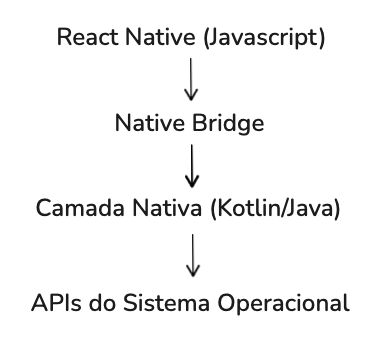
\includegraphics[width=0.5\textwidth]{figuras/Arquitetura-Modulo-Nativo.png}
\end{figure}


\subsection{Módulo Nativo de Monitoramento de Tempo de Tela}
O Android fornece nativamente a classe UsageStatsManager, que permite consultar o tempo que aplicativos ficaram em primeiro plano, obter estatísticas de uso por períodos específicos e listar aplicativos instalados e seus respectivos tempos de uso. Porém, para ter tal acesso é necessário ter a permissão especial PACKAGE-USAGE-STATS, que só pode ser concedida manualmente pelo usuário através das configurações do sistema. Para conseguir fazer tal acesso, a implementação foi dividida em três componentes principais


\subsubsection{Componente 1: ScreenTimeModule (Kotlin)}
O \textit{ScreenTimeModule} consiste em uma classe desenvolvida em \textit{Kotlin} que atua como intermediária entre a camada \textit{JavaScript} e as \textit{APIs} nativas do \textit{Android}. Esta classe herda de \textit{ReactContextBaseJavaModule}, classe base fornecida pelo \textit{React Native} para criação de módulos nativos.

A principal característica deste componente é a utilização da anotação @ReactMethod, que marca métodos como acessíveis a partir do código JavaScript. Cada método realiza uma operação específica relacionada ao monitoramento de tempo de tela, processando dados obtidos da API nativa e retornando resultados através de objetos Promise, garantindo comunicação assíncrona.

\textbf{Verificação de Permissões}: Consulta o sistema através da classe AppOpsManager para verificar se a aplicação possui a permissão PACKAGE-USAGE-STATS concedida, retornando um valor booleano.

\textbf{Solicitação de Permissão}: Direciona o usuário para a tela de configurações do sistema através de uma Intent (objeto de mensagem que solicita uma ação ao sistema Android) com ação ACTION-USAGE-ACCESS-SETTINGS, permitindo ativação manual da permissão.

\textbf{Cálculo de Tempo Diário}: Define um intervalo temporal da meia-noite até o momento atual, consulta o UsageStatsManager e soma o atributo totalTimeInForeground de cada aplicativo, convertendo o resultado de milissegundos para minutos.

\textbf{Histórico Semanal}: Itera pelos sete dias anteriores, definindo intervalos de 00:00:00 até 23:59:59 para cada dia, consultando a API e agregando os tempos totais, retornando uma lista ordenada de datas e minutos.


\textbf{Tempo por Aplicativo}: Consulta a API para um período configurável, agrega manualmente dados de múltiplas entradas do mesmo aplicativo, utiliza o PackageManager para obter nomes legíveis, ordena por tempo de uso decrescente e retorna os vinte aplicativos mais utilizados. Todas essas operações utilizam classes e atributos oficiais da plataforma \textit{Android}, como \textit{UsageStatsManager}, \textit{AppOpsManager}, \textit{PackageManager} e o campo \textit{totalTimeInForeground}, descritos na documentação para desenvolvedores do sistema.\footnote{Android Developers. UsageStatsManager e APIs relacionadas. Disponível em: \url{https://developer.android.com/reference/android/app/usage/UsageStatsManager}. Acesso em: 18 fev. 2026.}
O diagrama de código correspondente a este componente encontra-se no Apêndice G (Figura \ref{fig:ScreenTimeModule}).


\subsubsection{Componente 2: ScreenTimePackage (Kotlin)}
O \textit{ScreenTimePackage} é responsável pelo registro do módulo nativo no \textit{React Native}. Esta classe implementa a interface \textit{ReactPackage}, sobrescrevendo o método \textit{createNativeModules} que retorna uma lista contendo a instância do \textit{ScreenTimeModule}.

O registro efetivo ocorre na classe MainApplication, no método getPackages, onde o ScreenTimePackage é adicionado à lista de pacotes. Após este registro, todos os métodos anotados com @ReactMethod tornam-se acessíveis através do objeto NativeModules na camada JavaScript.
O diagrama de código correspondente a este componente encontra-se no Apêndice G (Figura \ref{fig:ScreenTimePackage}).

\subsubsection{Componente 3: ScreenTimeService (Javascript)}
Esta camada de serviço encapsula e abstrai as chamadas aos métodos nativos, fornecendo uma interface de alto nível para a aplicação \textit{React Native}.

O serviço importa \textit{NativeModules} do \textit{React Native}, extrai o \textit{ScreenTimeModule} registrado e define interfaces \textit{TypeScript} que descrevem a estrutura dos dados retornados. Exporta métodos assíncronos que correspondem aos métodos nativos, retornando \textit{Promises} (objetos que representam a conclusão futura de uma tarefa assíncrona) tipadas. Esta abordagem proporciona \textit{autocomplete}, validação de tipos, centralização de acesso e facilita manutenção sem modificar código nativo. Os conceitos de \textit{Promise}, \textit{NativeModules} e \textit{Firestore} seguem, respectivamente, a especificação de \textit{JavaScript}, a documentação oficial do \textit{React Native} e a documentação do \textit{Firebase}.\footnote{ECMA International. ECMAScript Language Specification. Disponível em: \url{https://tc39.es/ecma262/}. Acesso em: 18 fev. 2026.; React Native. Native Modules. Disponível em: \url{https://reactnative.dev/docs/native-modules-intro}. Acesso em: 18 fev. 2026.; Firebase. Cloud Firestore. Disponível em: \url{https://firebase.google.com/products/firestore}. Acesso em: 18 fev. 2026.}
O diagrama de código correspondente a este serviço encontra-se no Apêndice G (Figura \ref{fig:ScreenTimeService}).

\subsection{Regras de segurança}
Para garantir que o backend do Desconecta seja seguro, a estrutura do Firestore foi configurada usando regras que seguem o princípio do privilégio mínimo. A ideia central é que o sistema valide a identidade de quem está fazendo a requisição antes de liberar qualquer dado. Na coleção de usuários, por exemplo, o acesso é restrito ao dono da conta; o sistema compara o UID da autenticação com o ID do documento, garantindo que ninguém consiga ler ou alterar perfis alheios.

Nas funcionalidades de interação, como os grupos e o feed, a lógica de permissões é um pouco mais detalhada para permitir a colaboração sem abrir mão da segurança. Qualquer usuário autenticado pode visualizar o conteúdo ou postar no feed, mas a edição e a exclusão são controladas: apenas o autor original ou um administrador do grupo têm esse poder. Para tornar essa verificação mais limpa e eficiente, foi implementada uma função que consulta dinamicamente o cargo do usuário dentro da lista de membros do grupo antes de autorizar a transação.

A proteção do banco de dados é finalizada com uma regra de bloqueio total para qualquer caminho que não tenha sido mapeado. Esse comportamento de barrar o acesso por padrão é fundamental para a segurança do projeto, pois garante que, mesmo que novas coleções sejam criadas no futuro, nenhum dado será exposto acidentalmente até que uma regra específica seja definida. Em termos práticos, as regras do Firestore restringem leitura e escrita a documentos cujo identificador esteja associado ao usuário autenticado e negam qualquer operação em caminhos genéricos que não tenham sido explicitamente autorizados.

O código completo das regras configuradas no console do Firestore encontra-se no Apêndice G (Figura \ref{fig:FirestoreRules}).

\subsection{Arquitetura de Grupos e Gamificação}